\documentclass[../main.tex]{subfiles}
\graphicspath{{\currfiledir}}
\begin{document}
\chapter{Terminology}
\todo{Write intro here. Purpose etc.}

\section{Grapheme}
\textcquote[204]{crystal2010}{Graphemes are the smallest units in a writing system capable of 
causing a contrast in meaning.}
In linguistics, graphemes are often placed in angle brackets, e.g. \grapheme{a} or \grapheme{b}.
Sometimes \emph{graphemes} are called \emph{signs}.
The term \emph{sign} and \emph{grapheme} are considered to be equivalent and 
interchangeable throughout this work.

\section{Graph and allograph}
\textcquote[204]{crystal2010}{Graphemes are abstract units which may adopt a variety of forms 
\elide Each of these possible forms is known as \emph{graphs}\elide
There is a vast amount of physical variation in the shapes of graphs that does not affect the 
underlying identity of the grapheme\elide 
When graphs are analyzed as variants of a grapheme, they are known as \emph{allographs}.}
The Maya script uses a lot of allographs.
For example, the syllable \syllabogram{u} can be written in many ways all having the same meaning 
(\Cref{fig:terminology-grapheme-u-allographs}).
\begin{center}
    
\includegraphics[width=\textwidth,keepaspectratio]{img/grapheme-u-allographs}
    \captionof{figure}{Some allographs of the grapheme \grapheme{u}}
    \label{fig:terminology-grapheme-u-allographs}
\end{center}

\section{Hieroglyph and glyph}
The term \emph{hieroglyph} and \emph{glyph} are not precise terms.
Both are used in epigraphic literature, to address a group of one or more graphemes.
\textcquote[1]{bricker1986}{A ``glyph'' is a sign that can occur alone or in combination with 
other signs}.
\textcquote[34]{knorozov1967}{A hieroglyph consists of several graphemes, which are joined 
in writing}. 
Both expressions are considered to be equivalent and interchangeable throughout this work.
\emph{Glyphs} can represent a syllable, a single word or even a whole phrase 
(\cite[23]{macrilooper2003}).

For example, the glyph (\Cref{fig:terminology-glyph-utzapaw}) consists of the 
graphemes \grapheme{u}, \grapheme{tz\glottalstop{}a} and \grapheme{wa} representing the phrase
\mayan{u tz\glottalstop{}apaw}, ``she/he erects it''.
% LTeX: enabled=false
The glyph (\Cref{fig:terminology-glyph-ixwinikhaabajaw}) consisting of the 
graphemes \grapheme{ix}, \grapheme{winikhaab} and \grapheme{ajaw}
and represents the noble title \mayan{ix winikhaab ajaw}, ``Ruler Lady Winikhaab''.
\begin{figure}
    \centering
    \subfloat[][]{
        \centering
        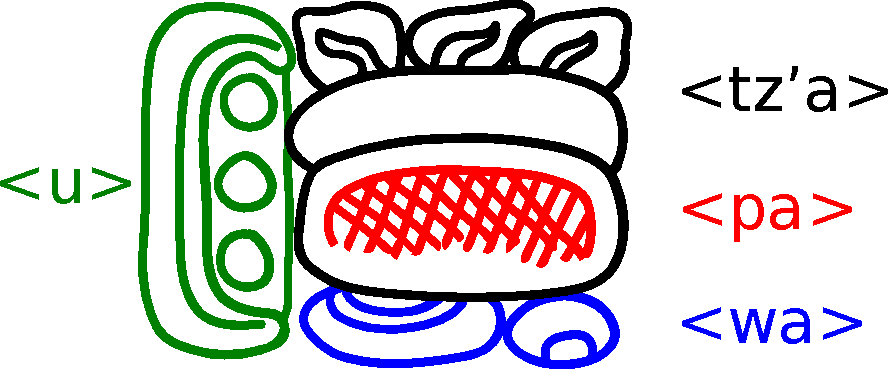
\includegraphics[height=\glyphblockheight]{img/glyphs-utzapaw}
        \label{fig:terminology-glyph-utzapaw}
    }
    \subfloat[][]{
        \centering
        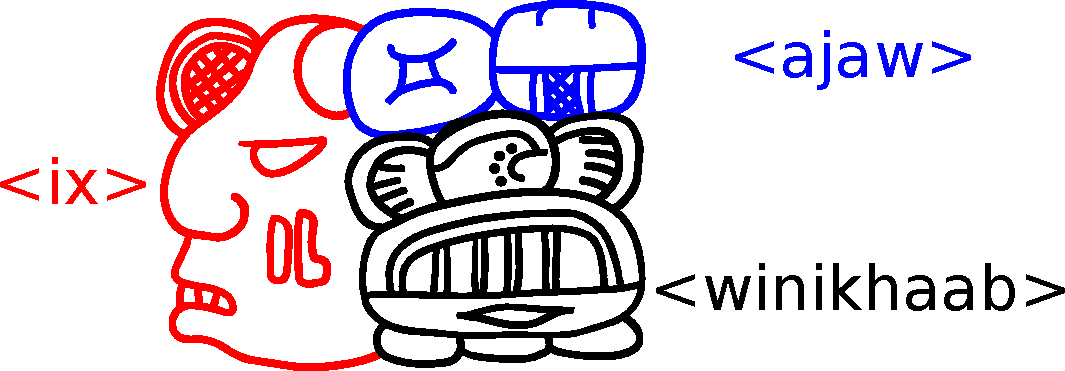
\includegraphics[height=\glyphblockheight]{img/glyphs-ixwinikhaabajaw}
        \label{fig:terminology-glyph-ixwinikhaabajaw}
    }
    \caption[Sample glyphs]{Sample glyphs: graphemes are distinguished by different colors.\\
            \subref{fig:terminology-glyph-utzapaw} \mayan{u tz\glottalstop{}apaw};
            \subref{fig:terminology-glyph-ixwinikhaabajaw} \mayan{ix winikhaab ajaw} 
            (\authordrawings).}
\end{figure}
% LTeX: enabled=true

\section{Glyph block and collocation}
One or more \emph{glyphs} are usually arranged in regular rectangular shapes called a 
\emph{glyph block}.
Sometimes they are also called \emph{collocation}.
\textcquote[1]{bricker1986}{A ``collocation'' is a group of signs that occupies a 
defined space, or block, in a hieroglyphic text.}
\textcquote[23]{macrilooper2003}{The rectangular shape of \emph{glyph blocks} results from 
the arrangement of texts into rows and columns}.
For example, Tonina monument 159 incoperates glyphs in rows and columns around tied up person 
(\Cref{fig:terminology-glyphs-in-rows-and-columns}).
% LTeX: enabled=false
\begin{center}
    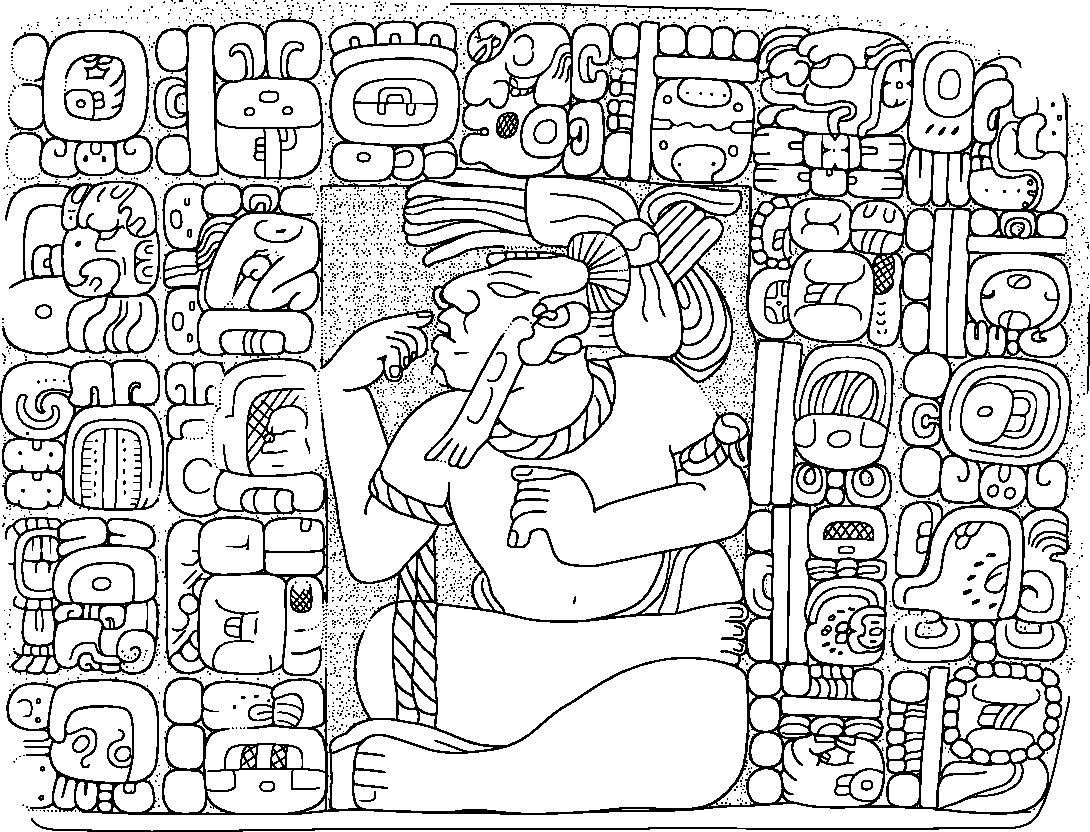
\includegraphics[width=\textwidth,keepaspectratio]{img/tonina-monument-159}
    \captionof{figure}{
        Glyph blocks arranged rows and columns. 
        Tonina monument 159 (Drawing by Guido Krempel, courtesy Coordinaci\'{o}n Nacional de 
        Conservaci\'{o}n del Patrimonio Cultural (CNCPC-INAH))}
    \label{fig:terminology-glyphs-in-rows-and-columns}
\end{center}
% LTeX: enabled=true

\section{Logogram and syllabogram}
A logogram is a sign which represents a word whereas a syllabogram is a sign which 
represents a syllable.

\section{Theory in decipherment}
\textcquote[2]{zender2017}{The type of writing system must be known}.
As Johannes Friedrich already stated:
\blockquote[{\cite[152]{friedrich1957}}]{The decipherment of any unknown script or language 
presupposes the availability of some clue or reference; nothing can be deciphered out of nothing. 
In those cases where one has absolutely no possibility available to link the unknown to 
something known, \elide no real or lasting result can be accomplished}

\subsection{Script typology}
For successful decipherment process, it is crucial to know the fundamental structure of the signs.
The type of the script can either be alphabetic, syllabic, logographic or a combination of them.
In order to classify an unknown writing system, the number of signs employed in the scripts
can hint what type of writing system one deals with.
% LTeX: enabled=false
Johannes Friedrich observed:
\blockquote[{\cite[152]{friedrich1957}}]{\elide~the number of the written symbols usually warrants a 
conclusion as to whether the script is alphabetic, a pure syllabary (as in the Cypriote) or a
mixture of ideographic word-signs and syllabic signs (like the cuneiform writing or the Hittite
hieroglyphic script). A script consisting of less than thirty signs will presumably turn out to
be alphabetic\elide~Scripts containing fifty, a hundred or even several hundred different symbols
may justifiably be regarded beforehand as more or less complicated syllabic systems of writing,
perhaps employing also word-signs\elide}.
% LTeX: enabled=true
Based on Ignace Gelb (\cite[115]{gelb1963}), Michael Coe (\cite[43]{coe1992}) compiled a list
of writing systems and compared their type with the number of distinct signs
(\Cref{table:terminology-writing-systems-comparison}).
\begin{table}[!ht]
    \centering
    \begin{tabular}{llc}
        \textbf{Type}                                                     & \textbf{Writing system} & \textbf{\# of signs} \\
        \multirow[t]{5}{20em}{\textbf{Logographic and Logosyllabic}\\
        Assigns a morpheme/word to each grapheme\\
        Logograms are either used for their semantic of syllabic values}  \\
                                                                          & Sumerian                & 600+ \\
                                                                          & Egyptian                & 2500 \\
                                                                          & Hittite Hieroglyphic    & 497 \\
                                                                          & Chinese                 & 5000+ \\        
        \\
        \multirow[t]{5}{20em}{\textbf{Syllabic}\\
        Assigns a syllable to each grapheme}                              \\
                                                                          & Persian                 & 40 \\
                                                                          & Linear B                & 87 \\
                                                                          & Cypriot                 & 56 \\
                                                                          & Cherokee                & 85 \\
        \\
        \multirow[t]{4}{20em}{\textbf{Abugida/Alphabetic Syllabary}\\ 
        Assigns a consonant to each grapheme\\
        Vowels or the absence of vowels are indicated by diacritics}      \\
                                                                          & Ethiopic                &  ca. 200 \\
                                                                          \\
                                                                          \\
        \\
        \multirow[t]{3}{20em}{\textbf{(Augmented) Abjad}\\
        Assigns a consonant to each grapheme\\
        In augmented abjad some vowels are added} \\
                                                                          & Phoenician              & 22 \\
                                                                          & Ugaritic                & 30 \\
        \\                                                                 
        \multirow[t]{8}{20em}{\textbf{(Augmented) Alphabet}\\
        Assigns a vowel or consonant to each grapheme}                    \\
                                                                          & English                 & 26 \\
                                                                          & Anglo-Saxon             & 31 \\
                                                                          & Sanskrit                & 35 \\
                                                                          & Etruscan                & 20 \\
                                                                          & Russian                 & 36 \\
                                                                          & Hebrew                  & 22 \\
                                                                          & Arabic                  & 28 \\
                                                                          & Coptic                  & 30 \\
    \end{tabular}
    \caption{Writing systems, their types and their number of distinct signs 
             (after~\cites[43]{coe1992}[730]{daniels1990}[88]{coulmas1991}{ritner1996})}
    \label{table:terminology-writing-systems-comparison}
\end{table}
So, in nutshell, to get a sense for the script type one can count the number of individual signs.
Then, it should be possible to narrow the number of possible script types by applying statistics of 
available writing systems (\Cref{table:terminology-writing-systems-comparison}).
The Maya text corpus is sufficiently big to do this with about 10,000 texts written on stone, wood, 
stucco, walls, pottery and four Post-Classic codices (\cite[151]{houstoncoe2003}).

\subsection{Corpus}
The database of texts (aka corpus) must be large enough so that sign catalogs can be created from it 
and analyzes of different text passages against each other allow effective comparisons 
(\cites[2]{zender2017}[44]{coe1992}).

\subsection{Language}
The language is crucial for any decipherment attempt.
If the languages died out or isn't spoken anymore, some ancestral or reconstructed 
version or some knowledge of the language family must be known (\cite[44]{coe1992}).
Marc Zender states \textcquote[3]{zender2017}{Absent some external evidence of the language, 
decipherment is impossible}.
However, Classic Maya --- the language of the Maya hieroglyphs ---  died out.
Although decipherment is challenging, it is possible to reconstruct texts by comparison 
with existing Maya languages as Christian Prager stated (\cite[6]{prager2018},my translation): 
\quotemytranslated[6]{prager2018}
% LTeX: enabled=false
{
    Es kann ausschließlich durch den Vergleich der 30 heute noch 
    gesprochenen Mayasprachen rekonstruiert werden. 
    Darüber hinaus ist vieles vom kulturellen Vokabular der vorspanischen Zeit als Folge der 
    Kolonisation verloren gegangen und bleibt bis heute eine große Herausforderung bei der 
    weiteren Entzifferung der Mayaschrift.
}
% LTeX: enabled=true
{
    It [Classic Maya] can only be reconstructed by comparing the 30 Mayan languages still 
    spoken today. 
    In addition, much of the cultural vocabulary of the pre-Hispanic period was lost as a result of 
    colonization and remains a major challenge in further decipherment of Maya writing 
    to this day.
}

\subsection{Cultural context}
\textcquote[44]{coe1992}{The cultural context of the script should be known, above all 
traditions and histories giving place-names, royal names and titles, and so forth.}
Well known place names, royal names or titles which occur in unknown script
play an important role in decipherment as they might hint how the fundamental mechanics of 
the writing system work.

\subsubsection{The Rosetta Stone}
One great example how royal names of titles helped to create an important insight of an unknown 
script, was the breakthrough Jean-Fran\c{c}ois Champollion had in deciphering the 
Egyptian hieroglyphs when analyzing the so-called Rosetta Stone which had a text written in 
three different writing systems, namely Greek, Demotic and Egyptian hieroglyphs.
Jean-Fran\c{c}ois Champollion focused on names of rulers which have been written both in 
Greek and in Egyptian hieroglyphs. 
Since Greek was well understood, the bilingual script helped him to compare the Greek writing with 
the Egyptian hieroglyphs.
Jean-Fran\c{c}ois Champollion realized, that in Egyptian hieroglyphs the names of personages 
are written in cartouches (\cite[215]{coulmas1991}).
One of the Greek names on the Rosetta Stone was \emph{Ptolemy}.
When comparing the name with hieroglyphs framed in cartouches, he deduced the phonetic writing 
of Ptolemy in Egyptian hieroglyphs (\Cref{fig:terminology-ptolemy-cartouche}).
This insight opened the possibility to assign phonetic values to hieroglyphic signs and 
played a major role to decipher Egyptian hieroglyphs. 
\begin{center}
    
\includegraphics[width=.7\textwidth,keepaspectratio]{img/ptolemy-cartouche}
    \captionof{figure}{Ptolemy written in Egyptian hieroglyphs (read from right to left) with 
                       phonetic decipherment (\authordrawings)}
    \label{fig:terminology-ptolemy-cartouche}
\end{center}

\subsubsection{Maya rulers of \chichenitza}
David Kelley was able to show that names of Maya rulers occur in the inscriptions and in colonial
sources from the 16th century.
On several inscriptions in the temple of \chichenitza, Herman Beyer (\cite{beyer1937}) 
found several similar sign collocations.
David Kelley could proof that these sequences of signs actually represent a
name of a Maya ruler (\cite{kelley1962a}). 
With the help of Landa's abecedary (\Cref{fig:terminology-landa-relacion-folio-45r}) and 
Yuri Knorozov decipherments (\cite{knorozov1967}) David Kelley found that these sign collocations 
denote the name of the Maya ruler \kakupakal 
(\cite[304-5]{kelley1962c}).
When he cross-referenced this name (\cite[\ppno~259--266]{kelley1968}) with the book of 
Chilam Balam of Chumayel 
--- one of several books from the colonial time written in Yucatec Maya and Latin letters ---
he discovered that on page 43r a person of high rank named \mayan{Kakupakal} is mentioned 
(\Cref{fig:terminology-chilam-balam-kakupakal}), 
translation by Ralph Roys (\cite[51,141]{roys1933}):
% LTeX: enabled=false
\begin{quote}
    Tu uucpiz tun Uaxac Ahau u katunil, laix u katunil cimci Chakanputin tumen 
    Kak-u-pacal yetel Tec Uilue.[In the seventh tun of Katun 8 Ahau, this was the katun when 
    Chakanputun perished at the hands of Kak-u-pacal and Tec Uilu[e].]
\end{quote}
% LTeX: enabled=true
Even though the identity of \mayan{Kakupakal} from the colonial sources and \kakupakal from the 
inscriptions in \chichenitza is doubtful, reading a Maya ruler's phonetically and the fact that 
both figures lived in the same region of \chichenitza encouraged the phonetic approach 
in the decipherment of Maya hieroglyphs.

% LTeX: enabled=false
\begin{figure}
    \centering
    \subfloat[][]{
        \centering
        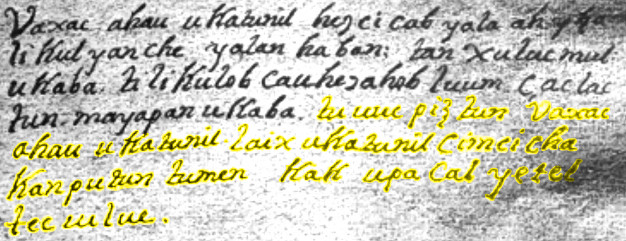
\includegraphics[width=0.60\textwidth]{img/chilam-balam-kakupakal}
        \label{fig:terminology-chilam-balam-kakupakal}
    }
    \subfloat[][]{
        \centering
        
\includegraphics[width=0.30\textwidth]{img/chichen-itza-monjas-lintel-2-kakupakal}
        \label{fig:terminology-chichen-itza-monjas-lintel-2-kakupakal}
    }
    \caption[\kakupakal in the colonial sources and inscriptions]
             {The name \kakupakal in the colonial sources and 
             in the inscriptions of \chichenitza.
             \subref{fig:terminology-chilam-balam-kakupakal} page 43r from the book of 
             Chilam Balam of Chumayel.
             \subref{fig:terminology-chichen-itza-monjas-lintel-2-kakupakal}
             Hieroglyphic writing from \chichenitza Monjas Lintel 2 (B1) (\authordrawings).}
\end{figure}
% LTeX: enabled=true

\subsection{Bilingual, biscript, or similar constraint}
Any clue as to what the content of the text might be is very important in deciphering an 
unknown script.
Bilingual scripts combining the unknown script with a well-known writing system helps to
verify the decipherment efforts (\cite[44]{coe1992}).
It can also be used to cross-reference readings of places, personage, titles etc. 
\textcquote[151]{houstoncoe2003}{If the script is logo-syllabic or heavily logographic, 
there should be accompanying pictorial references \elide to apply to the texts}.

Diego de Landa, a bishop who lived in Yucat\'{a}n in the 16th century, recorded aspects
of Maya writing in his work Relaci\'{o}n de las cosas de Yucat\'{a}n 
Even though his authorship is questionable (\cite{restallchuchiak2002}), this manuscript contains 
many aspects of Maya writing.
It contains vital information about the Maya calendars, the Maya signs for day names and month names
together with Spanish transcriptions.
It also contains the so-called ``Landa alphabet'' which basically represents a 
partial syllabary assigning a set of signs a phonetic value 
(\Cref{fig:terminology-landa-relacion-folio-45r}).
Additionally, the manuscript includes two sentences both written in Maya hieroglyphs and 
Latin letters.
\begin{center}
    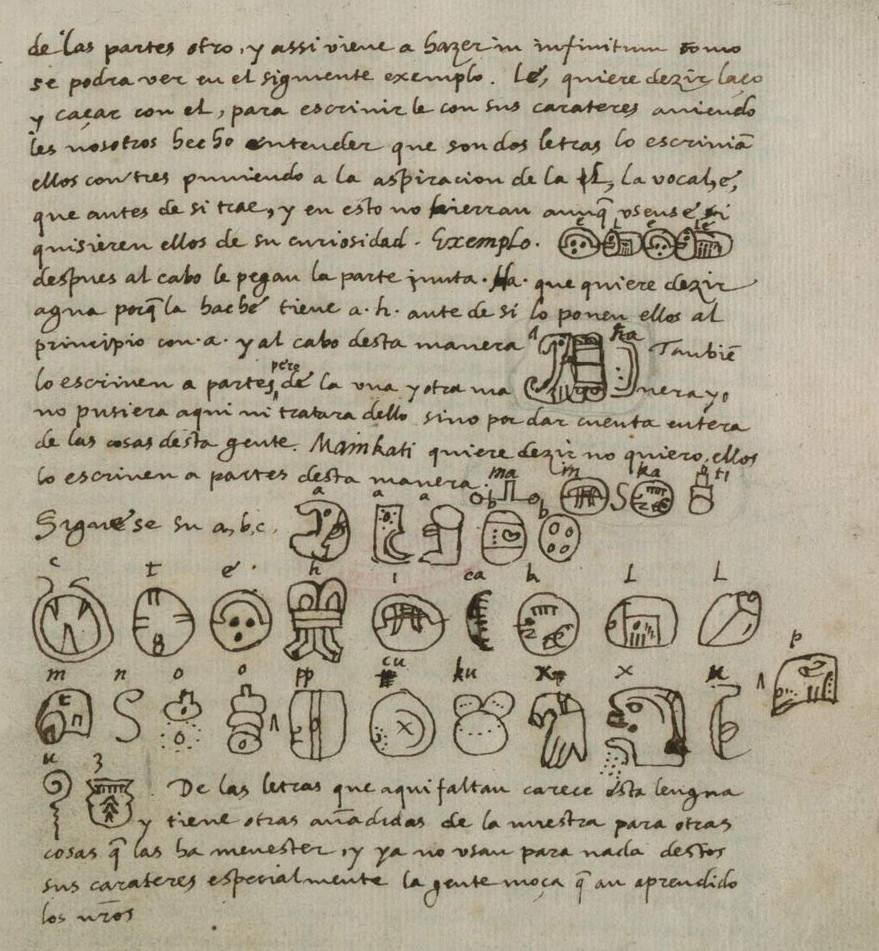
\includegraphics[width=0.8\textwidth,keepaspectratio]{img/landa-relacion-folio-45r}
    \captionof{figure}{Page 45r from Diego de Landa's manuscript containing the Landa alphabet, 
                       courtesy of the Real Academia de la Historia (\cite{landa1567})}
    \label{fig:terminology-landa-relacion-folio-45r}
\end{center}
Besides this bilingual resource, many Maya writings combine text with imagery.
\textcquote[152]{houstoncoe2003}{Realistic, narrative pictures accompany most texts, usually 
illustrating the actions of the people or gods talked about in the writing.}

\section{Cataloging of signs}
One of the first steps to analyze an unknown writing system, is to identify distinctive graphemes 
and their allographs. 
In the past, several sign catalogs have been proposed.
Yuri Knorozov created a sign catalog in his work (\cite[109\psq]{knorozov1967}).
William E. Gates' and G\"unter Zimmermann's catalogs (\cites{gates1931}{zimmermann1956}) are 
based on the Maya codices but did not include the signs from the inscriptions 
(\cite[4]{thompson1962catalog}). 
Eric Thompson extended G\"unter Zimmermann's idea and categorized all signs into affixes, main signs 
(including animal heads) and portrait signs (\cite[4]{thompson1962catalog}).
His catalog covers the Maya codices, the monumental inscriptions and other writings 
(e.g.\ ceramics, vessels, bones).
All catalogs assigned a number to each sign/grapheme.
To distinguish between the different catalog systems, it is common to use a prefix in 
conjunction with the number.
So, for example, all Thompson numbers are labeled with the prefix ``T'', e.g. \thompson{510}.

In 2003, Martha J. Macri and Matthew G. Looper proposed a new system which assigns all graphemes
a code consisting of three digits (\cite[21,25]{macrilooper2003}).
The first two digits specifies the category of the sign 
(e.g. A for animals, M for signs with hands etc.) whereas the third digit is an arbitrary number
sequencing the different graphemes.

The project ``Text Database and Dictionary of Classic Mayan'' (abbr. TWKM) (\cite{twkm2014}) lead by 
Prof.\ Dr.\ Nikolai Grube of the Department of Anthropology of the Americas at the University of 
Bonn is currently compiling an updated and revisited version of Thompson's sign catalog.
% LTeX: enabled=false
Christian Prager states, \textcquote{prager2020}{we are currently evaluating and revising Eric 
Thompson’s Catalog of Maya Hieroglyphs (1962). 
We are critically scrutinizing his system with the help of his original grey cards and 
supplementing it with signs that were not included in Thompson’s original catalogue. 
Despite its known shortcomings and incompleteness, his catalogue is still regarded as the 
standard work for Maya epigraphers, which is why we adopt Thompson’s nomenclature while 
removing misclassifications and duplicates, merging graph variants under a common nomenclature, 
and adding new signs or allographs to the sign index in sequence, starting with the number 1500.}
% LTeX: enabled=true

\subsection{Problems and limitations}
Having all these sign catalogs are a huge help to systematically analyze any writing system.
It is especially important when the writing system cannot be read.
As one could see above, researchers assign codes or numbers to address individual or 
even groups of signs.
Therefore, identifying graphemes are crucial to systematically build up a sign catalog.
Yet, determine them in an unknown writing system is challenging.
One way to approach this, is by segmenting the texts into distinct \emph{graphs}.
Researchers hereby followed the assumption that graphemes of a script are considered the same if 
they resemble each other in more features than either resembles any other.
\textcquote[34]{knorozov1967}{Two [signs] are identical when they are both composed of the same 
graphic elements\elide, whose drawing and disposition is sufficiently similar to allow them to 
be identified}.
However, if there is no control in terms of linguistics and content, 
this approach can be problematic.
Three major issues can occur when segmenting signs from an unknown writing system.
\begin{itemize}
    \item Allographs are interpreted as separate graphemes.
    \item Graphemes with distinct phonetic value and meanings are interpreted as allographs.
    \item Complex graphemes are split into its sub-graphemic components.
\end{itemize}
Especially in writing systems with many allographs like the Maya hieroglyphs,
allographs are sometimes not recognized and, instead, are interpreted as separate graphemes. 
Sometimes, signs are considered to be allographs because of their similarities, 
but, as later progress in decipherment has shown, were actually distinct graphemes.
Eric Thompson (\cite[12\psq]{thompson1962catalog}) recognized the method of segmentation as 
a potential source of false conclusions.
David Kelley (\cite{kelley1962b}) was able to show in his review of Thompson's sign catalog that
some T-numbers represent more than one grapheme and some T-numbers are allographs of another.
For example \thompson{683a} and \thompson{T683b} (\Cref{fig:terminology-t683a-t683b}) are
distinct graphemes whereas \thompson{589} and \thompson{T607} (\Cref{fig:terminology-t589-t607})
represent the same grapheme.
% LTeX: enabled=false
\begin{figure}
    \centering
    \subfloat[][]{
        \centering
        
\includegraphics[height=\glyphblockheight]{img/T683a-T683b}
        \label{fig:terminology-t683a-t683b}
    }
    \subfloat[][]{
        \centering
        
\includegraphics[height=\glyphblockheight]{img/T589-T607}
        \label{fig:terminology-t589-t607}
    }
    \caption[Questionable T-number assignment in Thompson's catalog]{Questionable T-number 
            assignment in Thompson's catalog (after Kelley).
            \subref{fig:terminology-t683a-t683b} \grapheme{winik} and \grapheme{ja} 
            assigned to \thompson{683};
            \subref{fig:terminology-t589-t607} \grapheme{ho} assigned to \thompson{589} and 
            \thompson{607} (\authordrawings).}
\end{figure}
% LTeX: enabled=true
Despite merging unrelated graphs or separating allographs which actually belong to each other,
the Maya writing system also utilizes graphemes which consist of two or more subgraphemic 
components.
Those complex graphemes might not be recognized and therefore only its components are registered
as graphemes.
One of those complex graphemes, is the grapheme \grapheme{pas} ``dawn'' 
(\Cref{fig:terminology-glyph-pas}) which is built from
grapheme \grapheme{chan} ``sky'' (\Cref{fig:terminology-glyph-chan}), 
grapheme \grapheme{k\glottalstop} ``k\glottalstop{}in'' (\Cref{fig:terminology-glyph-kin}) and
grapheme \grapheme{kab} ``earth'' (\Cref{fig:terminology-glyph-kab}).
It can be found, for example, on Tikal Temple IV, Lintel 2 A7.
All three components are graphemes themselves, but in combination they form the complex 
grapheme \grapheme{pas} with its own phonetic value and meaning.
This grapheme doesn't show up in Thompson's sign catalog.
Later revisions and new catalogs like Macri and Looper (\cite{macrilooper2003}) added it as
separate grapheme and assigned it the code ZX2.
% LTeX: enabled=false
\begin{figure}
    \centering
    \subfloat[][]{
        \centering
        
\includegraphics[height=\glyphblockheight]{img/grapheme-PAS}
        \label{fig:terminology-glyph-pas}
    }
    \subfloat[][]{
        \centering
        
\includegraphics[height=\glyphblockheight]{img/grapheme-CHAN}
        \label{fig:terminology-glyph-chan}
    }
    \subfloat[][]{
        \centering
        
\includegraphics[height=\glyphblockheight]{img/grapheme-KIN}
        \label{fig:terminology-glyph-kin}
    }
    \subfloat[]{
        \centering
        
\includegraphics[height=\glyphblockheight]{img/grapheme-KAB}
        \label{fig:terminology-glyph-kab}
    }
    \caption[Grapheme \grapheme{pas}]{Grapheme \grapheme{pas}. Even though it consists of three 
             other graphemes, it represents a self-contained grapheme with separate phonetic and 
             meaning (\cite[139]{prager2018}).
             \subref{fig:terminology-glyph-pas} \grapheme{pas} ``dawn'';
             \subref{fig:terminology-glyph-chan} \grapheme{chan} ``sky'';
             \subref{fig:terminology-glyph-kin} \grapheme{k\glottalstop{}in} ``sun'';
             \subref{fig:terminology-glyph-kab} \grapheme{kab} ``earth'' (\authordrawings).}
\end{figure}
% LTeX: enabled=true

\section{Mesoamerican chronology}
Researchers divide the history pre-Columbian Mesoamerica into several time periods 
(\cite{mendoza2001}):

\begin{itemize}
    \item The Paleo-Indian (first human habitation until 3500 BCE),
    \item the Archaic (before 2600 BCE),
    \item the Preclassic or Formative (2500 BCE --- 250 CE),
    \item the Classic (250 --- 900 CE)
    \item the Postclassic (900 --- 1521 CE)
    \item and the Colonial Period (1521 --- 1821)
\end{itemize}
The periodization of Mesoamerica is based on archaeological and architectural observations,
as well as on studies of the material culture and art.
Originally, it was not anchored to an absolute chronology.
It was rather based on the relative associations of cultural materials that had presumed or 
even known age.
The Classic period was eventually defined once the Maya calendar could be associated 
with Gregorian calendar.
The earliest monuments in the Classic appear around 300 CE and the latest ones around 900 CE framing
the period span of the Classic period between 300 CE and 900 CE\@.
Maya civilization before 300 CE has been coined Preclassic whereas Maya civilization
after 900 CE until the arrival of the first Spaniards is called Postclassic.
The Colonial period ended with the Mexican independence in 1821 ((\cite{mendoza2001})).

\section{The language of Maya Hieroglyphs}
The language of the Maya hieroglyphs is called ``Classic Mayan''.
The term ``Classic Mayan'' refers to the language used in inscriptions and writings
spanning from the early Preclassic until the time of the Spanish conquest.
After decades of close collaboration of many Epigraphers, linguists, art historians and 
archeologists it became possible to develop a deeper understanding of the language in the Maya 
texts and to analysis its grammar, syntax and general structure (\cite{lawstuart2017}).
Mayanists came to the conclusion that the Maya texts are written in
cohesive and consistent form suggesting that the language of these texts are based on
a common language.
This section gives just a short introduction.
For a more detailed explanation, please refer to the chapter ``Classic Mayan'' 
(\Cref{chap:classic-mayan}).

\subsection{Basic structure}
Classic Mayan and modern Mayan languages alike have a word other which usually follows
the verb-object-subject structure (\cite[24]{kettunenhelmke2020}).
In non-transitive sentences the pattern is verb-subject.
When a date is involved, the date comes first like so: date-verb-(object-)subject

\subsection{Phonology}
In Classic Maya, there are five different vowels and twenty distinct consonants.
The vowels are: \mayan{a}, \mayan{e}, \mayan{i}, \mayan{o} and \mayan{u}.
The consonants consist of values with and without glottal stop ('):
% LTeX: enabled=false
\mayan{b}, \mayan{ch}, \mayan{ch'}, \mayan{h}, \mayan{j}, 
\mayan{k}, \mayan{k'}, \mayan{l}, \mayan{m}, \mayan{n}, 
\mayan{p}, \mayan{p'}, \mayan{s}, \mayan{t}, \mayan{t'},
\mayan{tz}, \mayan{tz'}, \mayan{w}, \mayan{x}, and \mayan{y}.
% LTeX: enabled=true
\Cref{table:terminology-phonemes-vowels} and  \cref{table:terminology-phonemes-consonants} 
describe the phonetic values as-well as the orthography used throughout this work.
The writing conventions are based on the orthography proposed by 
Academia de Lenguas Mayas de Guatemala (\cite{instituto1988}).
% LTeX: enabled=false
\begin{table}[!ht]
    \centering
    \begin{tabular}{cc|cc|cc}
        Notation & IPA           & Notation & IPA            & Notation & IPA \\
        \hline
        a        & \textipa{[a]} & aa       & \textipa{[a:]} & \"a      & \textipa{[5]}\\
        e        & \textipa{[e]} & ee       & \textipa{[e:]} & \"e      & \textipa{[E]}\\
        i        & \textipa{[i]} & ii       & \textipa{[i:]} & \"{\i}   & \textipa{[I]}\\
        o        & \textipa{[o]} & oo       & \textipa{[o:]} & \"o      & \textipa{[\textlowering{7]}}\\
        u        & \textipa{[u]} & uu       & \textipa{[u:]} & \"u      & \textipa{[U]}
    \end{tabular}
    \caption{Orthography and phonemes for vowels} 
    \label{table:terminology-phonemes-vowels}
\end{table}
% LTeX: enabled=true
% LTeX: enabled=false
\begin{table}[!ht]
    \centering
    \begin{tabular}{cc|cc|cc|cc|cc}
        Symbol & IPA                & Symbol & IPA                          & Symbol & IPA                           & Symbol & IPA           & Symbol & IPA \\
        \hline     
        b      & \textipa{[b]}      & ch     & \textipa{[\t{\textteshlig}]} & ch'    & \textipa{[\t{\textteshlig}']} & h      & \textipa{[h]} & j      & \textipa{[X]}\\
        k      & \textipa{[k]}      & k'     & \textipa{[k']}               & l      & \textipa{[l]}                 & m      & \textipa{[m]} & n      & \textipa{[n]}\\
        p      & \textipa{[p]}      & p'     & \textipa{[p']}               & s      & \textipa{[s]}                 & t      & \textipa{[t]} & t'     & \textipa{[t']}\\
        tz     & \textipa{[\t{ts}]} & tz'    & \textipa{[\t{ts}']}          & w      & \textipa{[w]}                 & x      & \textipa{[S]} & y      & \textipa{[j]}\\
        \multicolumn{10}{l}{Glottal stop: ' \textipa{[P]}}
    \end{tabular}
    \caption{Orthography and phonemes for consonants} 
    \label{table:terminology-phonemes-consonants}
\end{table}
% LTeX: enabled=true

Vowels are usually abbreviated with \emph{V}, whereas consonants are abbreviated with \emph{C}.
Long vowels are usually written with a double vowel VV (e.g. \mayan{aa}).
Aspirated vowels have an affixed \mayan{h} which forms Vh.
Glottalized vowels are written as V' and rearticulated glottalized vowels as V'V.
In Maya literature, configurations like VV, Vh, V', V'V are usually called \emph{complex voxels} 
(\cite[276]{houstonstuartrobertson1998}):
% LTeX: enabled=false
\begin{itemize}
    \item VV\@: long vowels 
          (e.g. \mayan{tuun} --- \english{stone}, \mayan{muuch} --- \english{toad})
    \item Vh: aspirated vowel 
          (e.g. \mayan{nahb} --- \english{lake}, e.g. \mayan{ahk} --- \english{turtle})
    \item V\glottalstop: glottalized vowel
          (e.g. \mayan{k\glottalstop{}in} --- \english{sun}, 
           e.g. \mayan{ch'\glottalstop{}ok} --- \english{youngster})
    \item V\glottalstop{}V rearticulated glottalized vowel
          (e.g. \mayan{bu\glottalstop{}ul} --- \english{bean}, 
           e.g. \mayan{ha\glottalstop{}al} --- \english{waterlike})
\end{itemize}
% LTeX: enabled=true

\section{Analysis of hieroglyphic texts}
\todo{Everything}

\subsection{Transliteration of Maya signs}
In the study of writing systems, transliteration describes the conversion of one 
writing system into another (\cite[494]{crystal2008}).
Transliteration in Maya studies refers to the conversion of Maya writing into the Latin alphabet.
The type of sign (logogram/syllabogram) and in some cases the way of drawing is also encoded.
Every sign is converted separately.
Signs belong contextually to the same compound are connected via hyphens. 
This work uses the long-standing convention for transliterating 
Maya signs (\cite{jamesjusteson1984}).
\begin{itemize}
    \item Transliterations of logograms are written in uppercase, bold letters 
          (e.g. \cref{fig:terminology-chak-balam}).
    \item Graphemes which represent syllables aka syllabograms are represented in 
          lowercase, bold letters (e.g. \cref{fig:terminology-pa-ka-la}).
    \item Roman parenthesis enclose parts of a sign's transliteration which are not pronounced.
          For example, the name \emph{Pakal} when written with syllabograms only would be 
          transliterated.
          % LTeX: enabled=false
          \transliteration{\syllabogram{pa}-\syllabogram{ka}-\syllabogram{l(a)}}
          (\cref{fig:terminology-pa-ka-la}).
          % LTeX: enabled=true
    \item Question marks are placed after a transliterated syllabogram or a 
          logogram when the reading is questionable or uncertain 
          (e.g. \cref{fig:terminology-ta-ix-ajaw-wa}).
    \item Signs which do not appear in the text, but are reconstructed 
          --- contextually or by comparison of parallel texts --- are preceded by an asterisk
          (e.g. \cref{fig:terminology-ta-ix-ajaw-wa}).
    \item Fused signs are written in their-order of reading.
    \item Signs with infixed graphemes are written in their-order of reading and the infix is placed
          in square brackets 
          % LTeX: enabled=false
          (e.g. \transliteration{\syllabogram{ch\glottalstop{}o}\syllabogram{[ko]}}).
          % LTeX: enabled=true
    \item Signs of unknown value are either represented by Thompson codes or codes of the 
          revised version of Macri and Looper/Vail (\cites{macrilooper2003}{macrivail2009}) 
          or by catalog codes from ``Text Database and Dictionary of Classic Mayan'' (TWKM).
\end{itemize}
% LTeX: enabled=false
\begin{figure}[ht]
    \centering
    \subfloat[][]{
        \centering
        
\includegraphics[height=\glyphblockheight]{img/pa-ka-la}
        \label{fig:terminology-pa-ka-la}
    }
    \subfloat[][]{
        \centering
        
\includegraphics[height=\glyphblockheight]{img/chak-balam}
        \label{fig:terminology-chak-balam}
    }
    \subfloat[][]{
        \centering
        
\includegraphics[height=\glyphblockheight]{img/ta-ix-ajaw-wa}
        \label{fig:terminology-ta-ix-ajaw-wa}
    }
    \caption[Transliteration examples]{Transliteration examples.
            \subref{fig:terminology-pa-ka-la} Syllabograms: 
            \transliteration{\syllabogram{pa}-\syllabogram{ka}-\syllabogram{l(a)}} 
            (Maya ruler \mayan{Pakal});
            \subref{fig:terminology-chak-balam} Logograms: 
            \transliteration{\logogram{CHAK}-\logogram{BALAM}} (\english{puma});
            \subref{fig:terminology-ta-ix-ajaw-wa} Uncertain reading of 
            \logogram{IX} (\english{Lady}) and reconstructed \logogram{AJAW} (\english{Ruler})
            \transliteration{\syllabogram{ta}-\logogram{IX}?-*\logogram{AJAW}-\syllabogram{wa} }
            (\authordrawings).}
\end{figure}
% LTeX: enabled=true

\subsection{Transcription of Maya texts}
Transcription describes the systematic and consistent method of writing down the sounds of speech.
For transcribing Maya texts, the following conventions are used (\cite[14]{kettunenhelmke2020}):
\begin{itemize}
    \item Transcriptions are represented in italics.
    \item Long vowels and glottal sounds are indicated without [square brackets]
    \item Reconstructed sounds based on historical, internal, or paleographic evidence are 
          represented in [square brackets]
\end{itemize}

\subsubsection{Narrow and broad transcriptions}
Transcriptions which are detailed and include a lot of features like aspiration or 
slight nasalization of the vowel are called \emph{narrow transcriptions}.
Narrow transcriptions can represent the exact pronunciation of a speaker, even small pronunciation 
details like dialect or accent. 
If transcriptions is less detailed, 
they are called \emph{broad transcriptions} (\cite[490]{crystal2008}).

For example, a narrow transcription of the English word \english{seat} would be 
% LTeX: enabled=false
\narrowtranscription{\textipa{si:t}}.
% LTeX: enabled=true
The broad transcription \widetranscription{\textipa{sit}} doesn't include 
the long vowel indicator \textipa{:}.

\subsubsection{Reconstruction of sounds}
Reconstructed sounds are based on historical, internal, or paleographic evidence.
Reconstructions by applying rules of (complex) orthography are not taken into account.
That implies that proposals like the disharmony hypothesis proposed by 
Houston et al. (\cites{lacadena2004}{houstonstuartrobertson1998}) do not contribute to the
phonetic reconstruction process.
The main reason is, that those hypotheses can not guarantee a certain reading and phonetic
assignment, and as such are challenged by Mayanists (\cite[7]{boot2009}).
For instance, complex vowels sometimes derived from disharmonic spellings in the script are
accepted if and only if those vowels can be reconstructed by means of other linguistic methods.

\subsubsection{Syncope}
Syncope refers to the process of deleting an inner vowel within a word (\cite[469]{crystal2008}).
In Ch'olan languages, the penultimate vowel for stems with more than two syllables is lost, 
provided that the loss does not result in an impermissible 
consonant cluster (\cite[86]{kaufman1984}).

% LTeX: enabled=false
For example, the mid-vowel \mayan{o} or \mayan{u} in the Mayan noun \mayan{ahk'ot?/ahk'ut} 
for the English word \english{dance} gets elided when the noun is verbalized.
The intransitive verb \mayan{ahk'taj} for \english{he/she danced} derived from the 
noun \mayan{ahk'ot?/ahk'ut} doesn't contain the inner vowel anymore.
The phoneme has been syncopated.
% LTeX: enabled=true

\subsubsection{Underspelling}
A syllable can roughly be segmented into three parts (\cite[468]{crystal2008}):
\begin{itemize}
    \item The opening segment of a syllable is called \emph{onset}.
    \item The central segment is called \emph{nucleus}.
    \item The \emph{coda} is the final sound group of a syllable and is the part of the 
          syllable that follows the nucleus.
\end{itemize}
Underspelling describes the possibility to omit the coda when recording text.
The reader knows implicitly how to read the word.
In the Maya corpus, especially consonants like n, l, y, w, j, or h are elided 
in the hieroglyphic texts (\cite[143-144]{lawstuart2017}).

\subsubsection{Phonetic complements and phonetic indicators}
Logo-syllabic writing systems can make use of phonetic complements and phonetic indicators to
add information on how signs should be read.
This is especially useful for signs having more than one phonetic or logographic meaning or value.
Such signs are called \emph{polyvalent} signs.

A phonetic indicator is one or more additional signs placed next to a polyvalent sign to
indicate which phonetic or logographic value is intended (\cite[56-57]{whittaker2009}).
Japanese, for example, borrowed the Chinese logographic writing system to record Japanese.
Since the phonetic value of logograms in Chinese is often quite different from Japanese, 
syllabic signs acting as phonetic indicators can be placed next to it to hint the phonetic reading.
% LTeX: enabled=false
In \Cref{fig:terminology-japanese-hon} the word \japanese{hon} is written with syllabic signs 
\texticon{img/japanese-ho} (\japanese{ho}) and \texticon{img/japanese-n} (\japanese{n})
placed on top.
% LTeX: enabled=true
Combined it helps the reader to read the word as \japanese{hon}.
% LTeX: enabled=false
\begin{figure}[h!]
    \centering
    \subfloat[][]{
        \centering
        
\includegraphics{img/japanese-hon}
        \label{fig:terminology-japanese-hon}
    }
    \subfloat[][]{
        \centering
        
\includegraphics{img/japanese-ho}
        \label{fig:terminology-japanese-ho}
    }
    \subfloat[][]{
        \centering
        
\includegraphics{img/japanese-n}
        \label{fig:terminology-japanese-n}
    }
    \caption[Japanese phonetic indicators]{Phonetic indicators helping to read the 
             logographic sign \subref{fig:terminology-japanese-hon} as \japanese{hon}.\\
            Syllabic sign \japanese{ho} \subref{fig:terminology-japanese-ho} and 
            syllabic sign \japanese{n} \subref{fig:terminology-japanese-n} indicate the reading.}
\end{figure}
% LTeX: enabled=true
A phonetic complement extends the phonetic reading of word or phrase around a polyvalent sign.
It, therefore, doesn't only indicate a phonetic or logographic reading, but also prefixes or
suffixes the polyvalent sign (\cite[56-57]{whittaker2009}).
For instance, several signs in Japanese have polyvalent properties.
% LTeX: enabled=false
The sign \texticon{img/japanese-sei} has several phonetic values.
It can stand for \japanese{sei}, \japanese{o} and \japanese{u} among others.
% LTeX: enabled=true
% LTeX: enabled=false
\begin{figure}[h!]
    \centering
    \subfloat[][]{
        \centering
        
\includegraphics{img/japanese-sei}
        \label{fig:terminology-japanese-sei}
    }
    \subfloat[][]{
        \centering
        
\includegraphics{img/japanese-u}
        \label{fig:terminology-japanese-u}
    }
    \subfloat[][]{
        \centering
        
\includegraphics{img/japanese-mu}
        \label{fig:terminology-japanese-mu}
    }
    \subfloat[][]{
        \centering
        
\includegraphics{img/japanese-umu}
        \label{fig:terminology-japanese-umu}
    }
    \subfloat[][]{
        \centering
        
\includegraphics{img/japanese-ou}
        \label{fig:terminology-japanese-ou}
    }
    \caption[Japanese phonetic complements]{Phonetic complements suffixing the
             polyvalent sign \subref{fig:terminology-japanese-sei}.
            Syllabic sign \japanese{u} \subref{fig:terminology-japanese-u} and 
            syllabic sign \japanese{mu} \subref{fig:terminology-japanese-mu} indicate the reading
            \japanese{ou} \subref{fig:terminology-japanese-ou} and 
            \japanese{umu} \subref{fig:terminology-japanese-umu}.}
\end{figure}
% LTeX: enabled=true
Signs can also be both, a phonetic indicator and a phonetic complement at the same time either
prefixing of suffixing the sign in question.

In the Maya writing system, additional signs related a polyvalent sign function 
as phonetic indicators and in most cases also as phonetic complements.
However, in Maya literature, those signs are way usually just called phonetic complements.
This work will also use the term phonetic complement as this commonly used in Maya research.
For instance, the polyvalent sign \thompson{528} can represent the syllable \syllabogram{ku} or the
logogram \logogram{TUN}.
For instance, in \cref{fig:terminology-jukub} \thompson{528} is read as \syllabogram{ku} to form
the Classic Mayan term \mayan{jukub} for English \english{canoe}.
By adding the syllable \syllabogram{ni}, a scribe could indicate that the polyvalent sign
should be read as the logogram \logogram{TUN}.
\Cref{fig:terminology-ut-k'al-tun-ni} shows how the Classic Mayan term \mayan{k'al tuun} 
for English \english{stone binding} can be written with \thompson{528} functioning as 
logogram \logogram{TUN}.

% LTeX: enabled=false
\begin{figure}[ht]
    \centering
    \subfloat[][]{
        \centering
        \includegraphics[height=\glyphblockheight]{img/logogram-TUN}
        \label{fig:terminology-logogram-tun}
    }
    \subfloat[][]{
        \centering
        
\includegraphics[height=\glyphblockheight]{img/jukub}
        \label{fig:terminology-jukub}
    }
    \subfloat[][]{
        \centering
        
\includegraphics[height=\glyphblockheight]{img/i-ut-k'al-tun-ni}
        \label{fig:terminology-ut-k'al-tun-ni}
    }
    \caption[Polyvalent sign \thompson{528}]{Polyvalent sign \thompson{528}.
            It can be read either as syllabogram \syllabogram{ku} or as logogram \logogram{TUN}.
            \subref{fig:terminology-logogram-tun}
            Standardized form for \thompson{528}
            (Drawings from https://classicmayan.org/zeichenkatalog)
            \subref{fig:terminology-jukub}
            \transliteration{\syllabogram{ju}-\syllabogram{ku}-\syllabogram{b(i)}}:
            Classic Mayan term \mayan{jukub} for English \english{canoe}
            (Piedras Negras Panel 2 hieroglyph A'3);
            \subref{fig:terminology-ut-k'al-tun-ni} 
            \transliteration{
                \syllabogram{i}-\syllabogram{u}-\syllabogram{t(i)} 
                \logogram{K'AL}-\logogram{TUN}-\syllabogram{n(i)}}:
            Classic Mayan \mayan{i uht k'al tuun} for 
            Engish \english{then it happened the stone binding}: 
            (Puerto Barrios altar hieroglyph G3); (\authordrawings)}
\end{figure}
% LTeX: enabled=true

In rare cases, logograms are used purely for phonetic purposes (\cite{stuart2020}).
For example, in \cref{fig:terminology-ak'-bi-ya-hu-li-ya}
logogram \logogram{AK'} for \english{turkey} is used to form the word \mayan{ahk'ab} or
the adverb \mayan{ahk'biiy} for \english{yesterday} respectively
even though the adverb \mayan{ahk'biiy} has nothing to do with \english{turkeys}.
% LTeX: enabled=false
\glyphanalysis
    {img/ak'-bi-ya-hu-li-ya}
    {\logogram{AK'}[\syllabogram{bi}]-\syllabogram{ya} 
    \syllabogram{hu}-\syllabogram{li}-\syllabogram{ya}}
    {ahk'biiy huliiy}
    {ahk'b-iiy hul-iiy}
    {night-PST arrive-PST}
    {yesterday it arrived}
    {Quirigua Stela F Monument 06 B06 (\authordrawings)}
    {fig:terminology-ak'-bi-ya-hu-li-ya}
% LTeX: enabled=true

\subsection{Morphological segmentation and analysis}
Morphological segmentation describes the process of dividing the (reconstructed) transcriptions into
morphemes.
Glossing or morphological analysis classifies the string of morphemes into morpheme categories 
and types.
The following examples show how a given hieroglyphic block or text is transliterated, transcribed,
morphological segmented and classified.
\newline
Examples:
% LTeX: enabled=false
\glyphanalysis
    {img/u-tz'a-pa-wa-tun-ni}
    {\syllabogram{u}-\syllabogram{tz'a}[\syllabogram{pa}]-\syllabogram{wa} 
    \logogram{TUN}-\syllabogram{ni}}
    {utz'a[h]paw tuun}
    {u-tz'a[h]p-aw-\zeromorpheme tuun}
    {3SE-erect-THM-3SA stone}
    {(s)he erected the stone}
    {Quirigua Monument 16 Ballcourt Plaza Q'02 (\authordrawings)}
    {fig:terminology-u-tz'a-pa-wa-tun-ni}
% LTeX: enabled=true
% LTeX: enabled=false
\glyphanalysis
    {img/ch'ak-ka-ja-u-k'ab}
    {\logogram{CH'AK}-\syllabogram{ka}-\syllabogram{ja}
    \syllabogram{u}-\logogram{K'AB}}
    {ch'a[h]kaj uk'ab}
    {ch'a[h]k-aj-\zeromorpheme uk'ab}
    {chop[PAS]-THM-3SA 3SE-hand}
    {his/her arm has been chopped off}
    {TNA Stucco Mural (\authordrawings)}
    {fig:terminology-ch'ak-ka-ja-u-k'ab}
% LTeX: enabled=true

Every morpheme can be categorized and characterized by a set of (brief) explanations in terms 
of grammatical significance. 
Usually, those attributes are shortened and abbreviated using a standardized list of 
glossing abbreviations.
A list of glossing abbreviations used throughout this work can be found in 
\cref{table:terminology-glossing-abbreviations}
% LTeX: enabled=false
\begin{table}[!ht]
    \centering
    \begin{tabular}{llll}
        \textbf{Gloss} & \textbf{Meaning}                                 & \textbf{Gloss} & \textbf{Meaning} \\
        \\
        ---            & Morpheme boundary                                & EG             & Emblem Glyph \\
        \zeromorpheme  & Zero morpheme                                    & FCL            & Feminine classifier \\               
                       &                                                  & INC            & Inchoative voice \\                                
        1SE            & 1\textsuperscript{st} person sg.errogative       & INS            & Instrumental suffix \\                   
        2SE            & 2\textsuperscript{nd} person sg.errogative       & IS             & Initial series \\ 
        3SE            & 3\textsuperscript{rd} person sg.errogative       & ISIG           & Initial series introductory glyph \\
        1PE            & 1\textsuperscript{st} person pl.errogative       & IV             & Intransitive verb \\                     
        2PE            & 2\textsuperscript{nd} person pl.errogative       & IVD            & Intransitive verb, derived \\            
        3PE            & 3\textsuperscript{rd} person pl.errogative       & LC             & Long count calendar \\ 
                       &                                                  & LOC            & Locative suffix \\                     
        1SA            & 1\textsuperscript{st} person sg.absolute         & MCL            & Masculine classifier \\                 
        2SA            & 2\textsuperscript{nd} person sg.absolute         & N              & Noun \\                                 
        3SA            & 3\textsuperscript{rd} person sg.absolute         & NCL            & Numerical classifier \\                 
        1PA            & 1\textsuperscript{st} person pl.absolute         & NUM            & Numeral \\                              
        2PA            & 2\textsuperscript{nd} person pl.absolute         & PAS            & Passive voice \\                        
        3PA            & 3\textsuperscript{rd} person pl.absolute         & PDI            & Posterior date indicator \\
                       &                                                  & PE             & Period ending \\
        ADI            & Anterior Date Indicator                          & PS             & Primary standard sequence \\
        ADJ            & Adjective                                        & PST            & Past tense \\
        ADV            & Adverb                                           & PV             & Positional verb \\         
        AFT            & Affective                                        & REL            & Relational suffix \\             
        APAS           & Antipassive voice                                & SUF            & Suffix (for unidentified suffixes) \\
        CLT            & Clitic                                           & THM            & Thematic suffix \\        
        CR             & Calendar round                                   & TV             & Transitive verb \\     
        DEM            & Demonstrative pronoun                            & *              & Reconstructed word or morpheme \\
        DN             & Distance number                                  & C              & Consonant \\
        DNIG           & Distance number intro glyph                      & V              & Vowel \\
    \end{tabular} 
    \caption{Glossing abbreviations used in morphological segmentation and morphological analysis}
    \label{table:terminology-glossing-abbreviations}
\end{table}
% LTeX: enabled=true

\end{document}
